\documentclass[10pt]{beamer}

\usetheme{metropolis}
\usepackage{appendixnumberbeamer}

\usepackage{booktabs}
\usepackage[scale=2]{ccicons}

\usepackage{pgfplots}
\usepgfplotslibrary{dateplot}
\newcommand{\ra}{\rightarrow}
\newcommand{\la}{\leftarrow}
\newcommand{\ua}{\uparrow}
\newcommand{\da}{\downarrow}
\renewcommand{\S}{\mathcal{S}}
\newcommand{\A}{\mathcal{A}}
\newcommand{\E}{\mathbf{E}}
\newcommand{\U}{\mathcal{U}}
\newcommand{\R}{\mathbb{R}}
\newcommand{\eqdef}{\stackrel{\cdot}{=}}
\newcommand{\tu}{\tilde{u}}
\newcommand{\tj}{\tilde{J}}
\newcommand{\tr}{\tilde{r}}
\newcommand{\minp}{(\min,+)}
\newcommand{\op}{\oplus}
\newcommand{\om}{\otimes}
\newcommand{\V}{\mathcal{V}}
\newcommand{\mb}{\mbox{ }}
\newcommand{\norm}[1]{\|#1\|}
\newcommand{\inorm}[1]{\|#1\|_{\infty}}
\newcommand{\snorm}[1]{\left\|#1\right\|}
\newcommand{\sinorm}[1]{\left\|#1\right\|_{\infty}}

\usepackage{caption}
\usepackage{subcaption}
\usepackage{pifont}

\usepackage{xspace}
\newcommand{\themename}{\textbf{\textsc{metropolis}}\xspace}

\title{Algorithms for Planning under Uncertainty}
%\subtitle{APU}
\date{\today}
\author{Chandrashekar Lakshminarayanan}
\institute{Reinforcement Learning \& Artifical Intelligence Group,\\University of Alberta}
% \titlegraphic{\hfill\includegraphics[height=1.5cm]{logo.pdf}}

\begin{document}

\maketitle

\begin{frame}{Overview}
  \setbeamertemplate{section in toc}[sections numbeorange]
  \tableofcontents[hideallsubsections]
\end{frame}

\begin{frame}[fragile]{Simple Example}
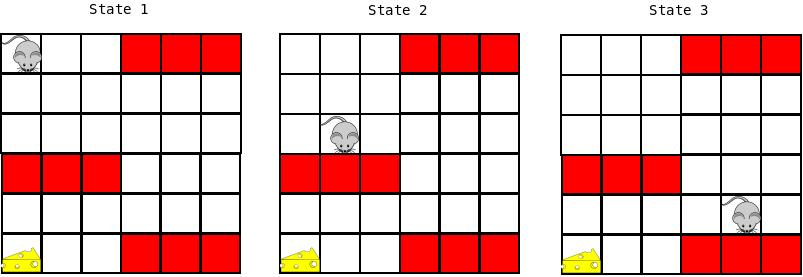
\includegraphics[scale=0.25]{mouse-allo.jpeg}
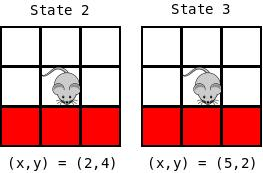
\includegraphics[scale=0.25]{mouse-states2.jpeg}
\color{black}
\begin{block}{}
\begin{itemize}
\item Map $u^*: s=(x,y)\ra action=\{\ra,\la,\ua,\da\}$
\item No Explicit Labels
\item Control via Noisy Feedback
\end{itemize}
\end{block}
\end{frame}

\begin{frame}[fragile]{Complex Systems}

$\mbox{ }$

\includegraphics[scale=0.125]{atari.jpg}
$\mbox{ }$
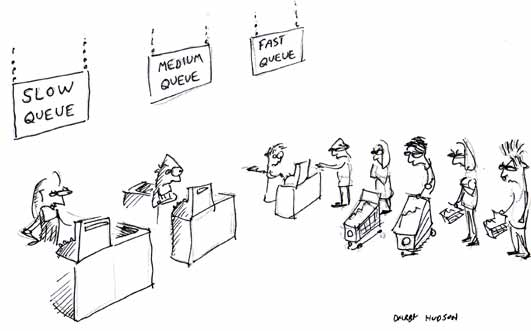
\includegraphics[scale=0.125]{queues1.jpg}
$\mbox{ }$
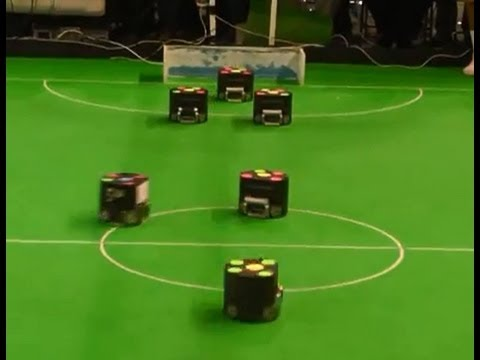
\includegraphics[scale=0.125]{robosoc.jpg}
$\mbox{ }$$\mbox{ }$
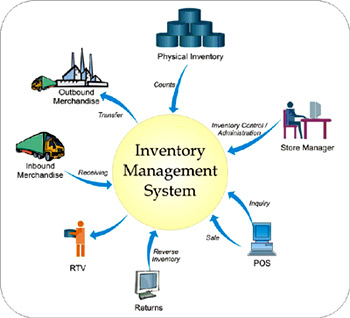
\includegraphics[scale=0.125]{invent.jpeg}
$\mbox{ }$\\
$\mbox{ }$
\quad Atari\quad\quad\quad\quad
$\mbox{ }$
Queues\quad\quad\quad\quad
$\mbox{ }$
 Robosoccer\quad\quad
$\mbox{ }$
Inventory
$\mbox{ }$\\
\quad\quad\quad\quad\quad\quad\quad
\quad\quad\quad\quad\quad\quad\quad
\quad\quad\quad\quad\quad\quad\quad
\quad\quad\quad
Control

\begin{figure}
\begin{table}
\begin{tabular}{cc}
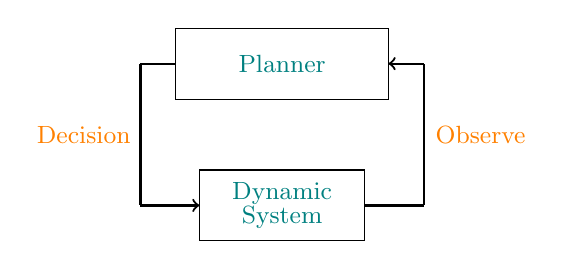
\begin{tikzpicture}[scale=0.6,font=\small,axis/.style={very thick, ->, >=sorangeth'}]

\draw [black=100](-2.25,-1.25) rectangle (2.25,0.25);
\node[teal] at(0,-0.5) {Planner};
%\node[black] at(0,-0.75) {};

\draw [black=100](-1.75,-4.25) rectangle (1.75,-2.75);
\node[teal] at(0,-3.25) {Dynamic};
\node[teal] at(0,-3.75) {System};

\node[orange] at(4.2,-2){\color{orange}{Observe}};


\node[orange] at(-4.2,-2){Decision};

\draw[thick,-](-2.25,-0.5)--(-3,-0.5);
\draw[thick,-](-3,-0.5)--(-3,-3.5);
\draw[thick,->](-3,-3.5)--(-1.75,-3.5);

\draw[thick,->](3,-0.5)--(2.25,-0.5);
\draw[thick,-](3,-3.5)--(3,-0.5);
\draw[thick,-](1.75,-3.5)--(3,-3.5);

\end{tikzpicture}
&
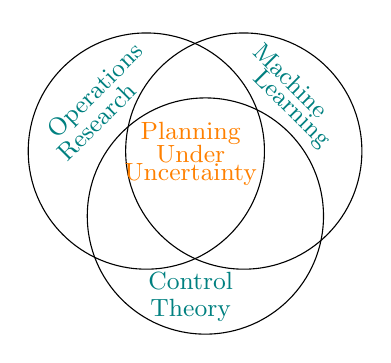
\begin{tikzpicture}[scale=0.75,font=\small,axis/.style={very thick, ->}]
\draw [] (0.9,0.5) circle (2);
\draw [] (-0.75,0.5) circle (2);
\draw [] (.25,-0.6) circle (2);
%\draw [] (-0.5,0.5) circle (2);
%\draw [] (0.5,-0.5) circle (2);
%\draw [] (-0.5,-0.5) circle (2);

\node[orange] at(0,0.8){Planning};

\node[orange] at(0,0.45){Under};
\node[orange] at(0,0.1){Uncertainty};

\node[teal,rotate=-45] at(1.7,1.7){Machine};
\node[teal,rotate=-45] at(1.7,1.2){Learning};

\node[teal,rotate=45] at(-1.6,1.5){Operations};
\node[teal,rotate=45] at(-1.6,1.0){Research};

\node[teal] at(-0,-1.7){Control};
\node[teal] at(-0,-2.2){Theory};
\end{tikzpicture}

\end{tabular}

\end{table}
%\caption*{No Explicit Labels; Control via Feedback }
\end{figure}


\end{frame}

\begin{frame}[fragile]{Challenge~I: {Curse-of-Dimensionality}}

\begin{itemize}
\item Huge State Space $\Rightarrow$  {\color{orange}{Exact Decision $u^*$ not possible}}
\item Compression by parameterization $\Rightarrow$ {\color{orange}{Approximate Decisions $\tilde{u}$}}
\end{itemize}

\begin{table}
\begin{tabular}{ccc}

\begin{minipage}{0.3\textwidth}
\begin{figure}
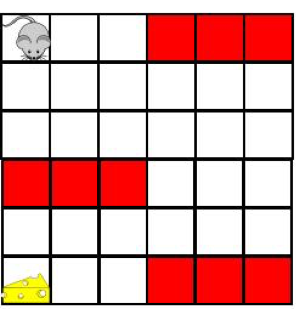
\includegraphics[scale=0.4]{mouse-single.png}
\caption*{Original}
\end{figure}
\end{minipage}
&
\begin{minipage}{0.3\textwidth}
\begin{figure}

\includegraphics[scale=0.4]{compress-mouse.png}
\caption*{Compressed }
\end{figure}
\end{minipage}
&
\begin{minipage}{0.3\textwidth}
\begin{block}{Open Question}
%{\color{orange}{Performance}}\\
{\color{orange}{How bad is $\tu$ in comparison to $u^*$?}}\\
\end{block}
\end{minipage}

\end{tabular}
\end{table}


\begin{block}{Keyword}
Approximate Dynamic Programming (ADP)
\end{block}

\end{frame}

\begin{frame}[fragile]{Challenge~II: {Lack of Model}}
\begin{itemize}
\item Noisy Sample Trajectories ({\color{orange}{$s_0-a_0-s_1-a_1-\cdots$}})
\item Adaptive Online updates({\color{orange}{$\theta(0),\theta(1),\ldots, \theta(t)$}})
\end{itemize}
\begin{table}
\begin{tabular}{cc}
\begin{minipage}{0.5\textwidth}
\begin{figure}
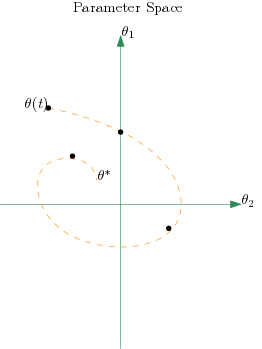
\includegraphics[scale=0.4]{traj.png}
\end{figure}
\end{minipage}
&
\begin{minipage}{0.5\textwidth}
\begin{block}{Open Question}
{\color{orange}{Stability?}}\\
{\color{orange}{$\theta(t)\ra \theta^*$ ?}}
\end{block}
\end{minipage}
\end{tabular}
\end{table}
\begin{block}{Keyword}
Reinforcement Learning; Stochastic Approximation
\end{block}

\end{frame}

\begin{frame}[fragile]{Research Contributions}
\textbf{\color{orange}{Developed ADP methods with provable performance guarantees}}
\begin{block}{Highlights}
\begin{itemize}
\item Novel basis in $(\min,+)$ algebra
\item Novel Monotone projection, Contraction Maps
\item Geometric conditions in linear optimization
\end{itemize}
\end{block}

\begin{block}{Publications}
Chandrashekar, L.; Bhatnagar, S., ``Approximate Dynamic Programming with $(\min,+)$ linear function approximation for Markov Decision Processes," $53^{rd}$ IEEE CDC, 2014\\
Chandrashekar, L.; Bhatnagar, S., ``A Generalized Reduced Linear Program for Markov Decision Processes," $29^{th}$ AAAI conference, 2015
\end{block}

\end{frame}
\begin{frame}[fragile]{Research Contributions}
\textbf{\color{orange}{Provided conditions that imply stability of multi-timescale stochastic approximation algorithms}}
\begin{block}{Highlights}
\begin{itemize}
\item Ordinary Differential Equation based analysis of Borkar et al
\item Umbrella result for various Reinforcement Learning algorithms
\end{itemize}
\end{block}

\begin{block}{Publication}
Chandrashekar, L. and  Bhatnagar, S. ``A Stability Criterion for Two Timescale Stochastic Approximation Schemes",  Automatica, 2017
\end{block}
\end{frame}
\begin{frame}[fragile]{Research Contributions}
\begin{block}{Crowd Sourcing}

Chandrashekar, L.;  Dubey, A.; Bhatnagar, S. and Chithralekha, B., ``A Markov Decision Process framework for porangeictable job completion times on crowdsourcing platforms", Proceedings of the Second {AAAI} Conference on Human Computation and Crowdsourcing, {HCOMP} 2014, Pittsburgh, Nov. 2-4, 2014
\end{block}
\begin{block}{Value Function}
Maity, R. K.; Chandrashekar, L.;  Padakandla, S.; Bhatnagar, S., `` Shaping Proto-Value Functions Using Rewards", European Conference on Artificial Intelligence 2016\\
\end{block}
\begin{block}{Constraint Sampling}
Chandrashekar, L.;  Bhatnagar, S and Szepesv\'{a}ri C., ``A Linearly Reduced Approximate Linear Program for Markov Decision Processes", submitted to IEEE Transactions on Automatic Control
\end{block}

\end{frame}

\section{Problem Setup}
\begin{frame}[fragile]{Markov Decision Process (MDP)}
Framework to cast problems of planning under uncertainty
\begin{block}{MDP}
\begin{itemize}
\item State space $\S=\{s^1,\ldots,s^n\}$
\item Action space $\A=\{a^1,\ldots,a^d\}$
\item Markovian Transition
\begin{align*}
Pr\{s_{t+1}=s'| s_t=s, a_t=a\}=p_a(s,s')
\end{align*}
\item Rewards $g_a(s)$ for action $a$ in state $s$
\item Policy: $u\colon \S\ra \A$ (induces a Markov chain with kernel $P_u$)
\item Value: $J_u(s)\eqdef \E\big[\sum_{t=0}^\infty \alpha^t g_{a_t}(s_t)|s_0=s,a_t=u(s_t)\big]$
\end{itemize}
\end{block}

\begin{tikzpicture}[overlay]
\node[black] at (10,5) {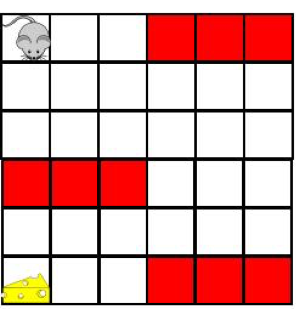
\includegraphics[scale=0.25]{mouse-single.png}};

\end{tikzpicture}


\end{frame}

\begin{frame}[fragile]{Dynamic Programming in a Nutshell}
\begin{itemize}
\item There are $|\A|^{|\S|}$ policies
\item Optimal Value: $J^*(s)\eqdef\max_{u}J_u(s),\,\forall s\in \S$
\item Greedy: {\color{orange}{Best = Current Best+ Future Best}}
\item Optimal Policy: $u^*(s)\eqdef \U(J^*) =\arg\max_{a\in \A} g_a(s)+\alpha p_a(s,\cdot)^\top J^*$
\item $J^*=TJ^*$, where $(TJ)(s)\eqdef\max_{a\in \A} g_a(s)+\alpha p_a(s,\cdot)^\top J$
\end{itemize}

\begin{block}{}
When model is given the problem boils down to computing $J^*(s),\,\forall s\in \S$
\end{block}

\begin{tikzpicture}[overlay]
\node[black] at (10,5) {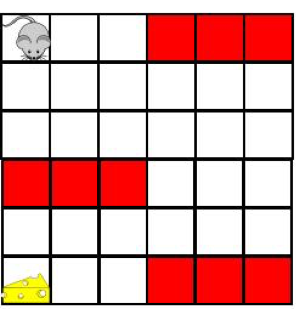
\includegraphics[scale=0.25]{mouse-single.png}};

\end{tikzpicture}


\end{frame}

\begin{frame}[fragile]{Basic Algorithms}
\begin{block}{Value Iteration}
\begin{center}
Power Method: $J_{t+1}=T J_t$
\end{center}
\end{block}
\begin{block}{Policy Iteration}
\begin{center}
Evaluation: $J_{u_t}=T_{u_t} J_{u_t}$\\
Improvement: $u_{t+1}=\U J_{u_t}$
\end{center}
\end{block}

\begin{block}{Linear Programming}
\begin{align*}
J^*&=\arg\min_{J\in \R^{\S}} c^\top J\\
&\quad s.t. J\geq TJ
\end{align*}
\end{block}
\begin{center}{Proof}
$L_\infty$ norm contraction property of $T$
\end{center}
\end{frame}


\begin{frame}[fragile]{Toy Grid World}

\begin{table}
\begin{tabular}{|c|c|c|}\hline
$\mb $&$\uparrow$	&$G$\\\hline
${\leftarrow}$	&$s$	&$\ra$\\\hline
$\mb$	&$\downarrow$	&$\mb$	\\\hline
\end{tabular}
\end{table}
\begin{itemize}
\item $S=X\times Y$, $A=\{\leftarrow,\rightarrow,\uparrow,\downarrow\}$, $\alpha=0.9$.
\item With $p=0.9$ move to desiorange position.
\item Reward at $G$ is $1$ otherwise $0$.
\end{itemize}

\begin{table}
\begin{tabular}{|c|c|c|}\hline
~$0$~	&~$0$~	&~$1$~\\\hline
$0$	&$0$	&$0$\\\hline
$0$ &$0$	&$0$\\\hline
\end{tabular}
\begin{tabular}{|c|c|c|}\hline
$0$	&$0.81$	&$1$\\\hline
$0$	&$0$	&$0.81$\\\hline
$0$ &$0$	&$0$\\\hline
\end{tabular}
\end{table}

\begin{table}
\begin{tabular}{|c|c|c|}\hline
$0.72$	&$1.53$	&$1.9$\\\hline
$0$	&$0.72$	&$1.53$\\\hline
$0$      &$0$	&$0.72$\\\hline
\end{tabular}
\begin{tabular}{|c|c|c|}\hline
$7.2$	&$8.1$	&$10$\\\hline
$6.56$	&$7.29$	&$8.1$\\\hline
$5.90$ &$6.56$	&$7.29$\\\hline
\end{tabular}
\end{table}
\begin{tikzpicture}[overlay]
\node[orange] at (4,4.25) {$TJ$};
\node[orange] at (6,4.25) {$T^2J$};

\node[orange] at (4,2.2) {$T^3J$};
\node[orange] at (6,2.2) {$J^*$};

\end{tikzpicture}


\end{frame}



\section{Approximate Dynamic Programming with provable performance guarantees}
\begin{frame}[fragile]{Approixmate Dynamic Programming (ADP)}
\begin{table}
\begin{tabular}{cc}
\begin{minipage}{0.5\textwidth}
\begin{block}{Why?}
\begin{itemize}
\item Curse-of-Dimensionality
\item Cannot compute exact $u^*$
\end{itemize}
\end{block}
\begin{block}{What?}
{\color{orange}{ADP= Compression + DP}}
\end{block}
\begin{block}{How?}
Compute $\tj\approx J^*$ and $\tu=\U \tj$
\end{block}
\begin{block}{Promise}
{\color{orange}{$\underbrace{||J_{\tilde{u}}-J^*||_\infty}_{\text{Performance Loss}} \leq \frac{2}{1-\alpha}\underbrace{||J^*-\tilde{J}||_\infty}_{\text{Value Error}}$}}
\end{block}
\end{minipage}
&
\begin{minipage}{0.5\textwidth}
\begin{table}
\begin{tabular}{ccc}

\begin{minipage}{0.3\textwidth}
\begin{figure}
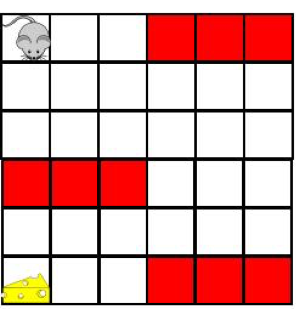
\includegraphics[scale=0.2]{mouse-single.png}
\caption*{DP}
\end{figure}
\end{minipage}
&
\begin{minipage}{0.3\textwidth}
\begin{figure}

\includegraphics[scale=0.2]{compress-mouse.png}
\caption*{ADP}
\end{figure}
\end{minipage}
&
\begin{minipage}{0.25\textwidth}
%\begin{block}{???}
%{\color{orange}{Performance}}\\
{\color{orange}{$\norm{J^*-J_{\tu}}$}}\\
%\end{block}
\end{minipage}
\end{tabular}
\end{table}

\end{minipage}
\end{tabular}
\end{table}
\end{frame}


\begin{frame}[fragile]{ADP in a nutshell}
How to compress?
\begin{itemize}
\item Parameterize the value function $J\in \Phi(r)$
\item Linear parameterization is popular $\Phi(r)=\Phi r$ ($\Phi$ is $|\S|\times k$ matrix $r\in \R^k$ is weight vector)
\item Pick $\tj=\Phi(\tr)\approx J^*$
\item Obtain $\tu=\U \tj$
\end{itemize}
\begin{center}
\begin{table}
\begin{tabular}{|c|c|}\hline
Exact DP& ADP \\ \hline
$u^*=\U J^*$    & $\tu=\U \tj$ \\ \hline
\end{tabular}
\end{table}
\end{center}
\begin{block}{Performance}

\end{block}
\end{frame}

\begin{frame}[fragile]{Compression+DP : Does it work?}
\begin{itemize}
\item Value Iteration{\color{orange}\ding{53}} $\Phi r_{t+1}= \Pi T (\Phi r_t)$ ({\color{orange}{No fixed point}})\footnote{$\Pi=\Phi (\Phi^\top \Phi)^{-1}\Phi$ is the projection. }

$\Pi T$ is not a contraction

\item {Policy Iteration}{\color{orange}\ding{53}}
\begin{align*}
&\Phi r_t=\Pi T_{u_t} \Phi J_{r_t} \\
&u_{t+1}=\U \Phi_{r_t}\text({\color{orange}{Poor~guarantee}})
\end{align*}

$\norm{\Phi r^*-J^*}_D\leq \frac{1}{1-\alpha}\norm{\Pi J^*-J^*}_D$
\item {Linear Programming}{\color{orange}\ding{53}}
\begin{align*}
\Phi r^*&=\arg\min_{r\in \R^{k}} c^\top \Phi r\\
&\quad s.t. \Phi r\geq T \Phi r ({\color{orange}{Large~Number~of~Constraints}})
\end{align*}
\end{itemize}
\end{frame}
\subsection{Tropical basis}
\begin{frame}[fragile]{Tropical Basis}
\begin{itemize}
\item A
\end{itemize}
\end{frame}
\begin{frame}

\begin{block}{}
\centering
\alert{Guarantees for AVI/API$^{\dagger}$}
\end{block}
\tiny
\begin{block}{}
$\dagger$Chandrashekar Lakshminarayanan and Shalabh Bhatnagar, Approximate Dynamic Programming with $\minp$ linear basis for Markov Decision Processes, CDC 2014
\end{block}
\end{frame}

\begin{frame}{$\minp$ Algebra}
\begin{block}{$\minp$ Linear Basis}
\vspace{-10pt}
\begin{align*}
\tilde{J}&=\min\{\phi_{1}+r(1),\ldots,\phi_{k}+r(k)\}
&=\Phi \om r
\end{align*}
\end{block}

\vspace{-10pt}
\begin{block}{Projection in $\minp$}
\vspace{-10pt}
\begin{align*}
\Pi_M J&=\{\min v \in \V | v \geq J\},
\end{align*}
where $V=\{\Phi \om r| r\in \R^k\}$ is the $\minp$ linear span of $\Phi$
\end{block}
\end{frame}

\begin{frame}{Projections in the $(\min,+)$ basis}
\begin{itemize}
\item $f(x)=x^2$
\item $a=(a(j),j=1,\ldots,5)=(-0.8,-0.4,0,0.4,0.8)$
\item $\phi_j(x)=2|x-a(j)|$
\item $\tilde{f}(x)=\min\{\phi_1(x)+r(1),\ldots,\phi_5(x)+r(5)\}$
\end{itemize}
\begin{figure}\label{illust}
\begin{tikzpicture}[scale=0.6]
\begin{axis}[
xlabel=x,
ylabel=f(x),
ymin=0,
ymax=1.5
]
\only<1-> {\addplot[smooth,orange] plot file {mfile/f.dat}};
\only<2-2> {\addplot[dashed,blue] plot file {mfile/fo1.dat}};
\only<2-2> {\addplot[dashed,blue] plot file {mfile/fo2.dat}};
\only<2-2> {\addplot[dashed,blue] plot file {mfile/fo3.dat}};
\only<2-2> {\addplot[dashed,blue] plot file {mfile/fo4.dat}};
\only<2-2> {\addplot[dashed,blue] plot file {mfile/fo5.dat}};
\only<3-> {\addplot[dashed,blue] plot file {mfile/f1.dat}};
\only<3-> {\addplot[dashed,blue] plot file {mfile/f2.dat}};
\only<3-> {\addplot[dashed,blue] plot file {mfile/f3.dat}};
\only<3-> {\addplot[dashed,blue] plot file {mfile/f4.dat}};
\only<3-> {\addplot[dashed,blue] plot file {mfile/f5.dat}};
\only<4-> {\addplot[smooth,black] plot file {mfile/fproj.dat}};
%   \addplot[dashed,black] plot file {mfile/f6.dat};
\end{axis}
\end{tikzpicture}
\caption{$(\min,+)$ LFA of $f(x)$}
\label{minptrans}
\end{figure}
\end{frame}

\begin{frame}
\frametitle{Contraction Map}
\begin{itemize}
\item {Monotonicity:} $\Pi_M J_1\geq \Pi_M J_2, \mb \forall$ $J_1\geq J_2$
\item {Shift:} $\Pi_M J_1= \Pi_M J_2+\mathbf{1}$ for $J_1\eqdef J_2+\mathbf{1}$
\item $\max$-norm contraction: $\Pi_M T$ is a contraction map in $\max$-norm
\end{itemize}
\end{frame}




\begin{frame}
\frametitle{Results}
\tikzstyle{na} = [baseline=-.5ex]

\begin{block}{Projected Bellman Equation}
\begin{align*}
\Phi \om r^*=\Pi_M T \Phi \om r^*
\end{align*}
\end{block}
\begin{tikzpicture}[overlay]
\visible<2->{
\node[orange] at (9,1) {Contraction in $L_\infty$!};
\draw[orange,thick] (5.6,1) circle(0.45);
}
\end{tikzpicture}
\vspace{-10pt}

\begin{block}{Main Theorem}
Let $\tilde{J}=\Phi \om r^*$ then
\begin{align*}
||J^*-\tilde{J}||_\infty&\leq \frac{2}{1-\alpha}\arg\min_r||J^*-\Phi\om r||_\infty
\end{align*}
\end{block}

\end{frame}
\begin{frame}{Results}
\begin{block}{}
$\mbox{ }$
$\mbox{ }$$\mbox{ }$
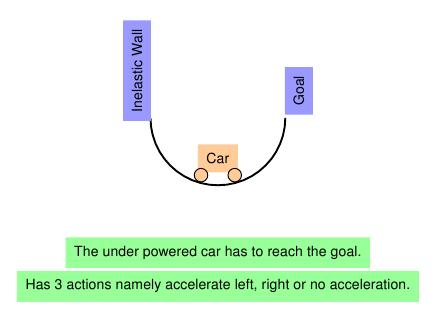
\includegraphics[scale=0.29]{mcarpic.jpeg}
$\mbox{ }$
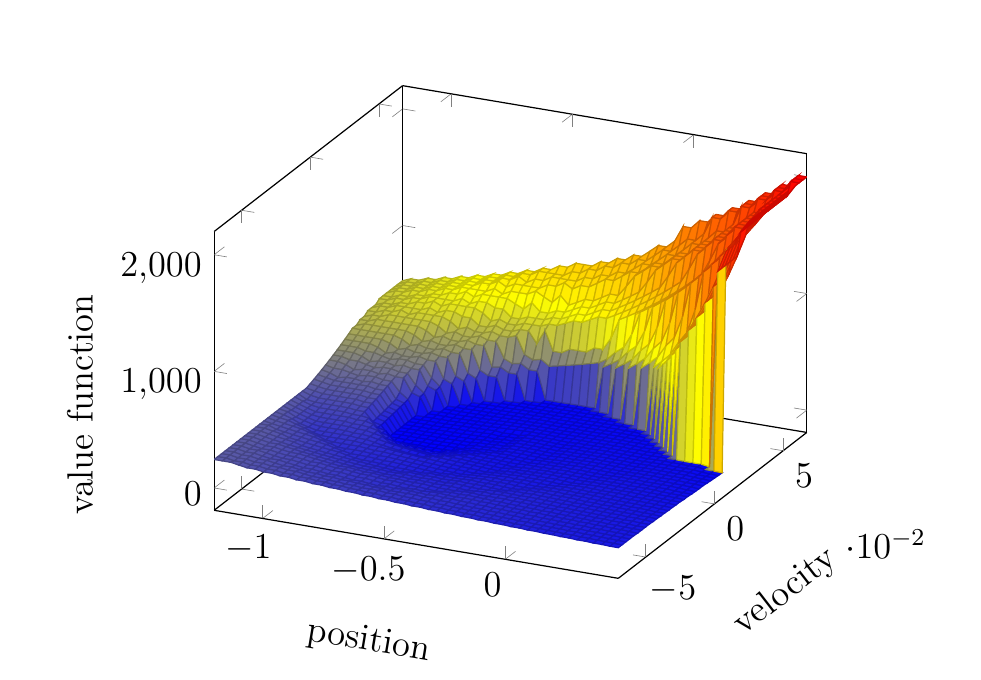
\includegraphics[scale=0.21]{actval.jpeg}\\
$\mbox{ }$\\
$\mbox{ }$
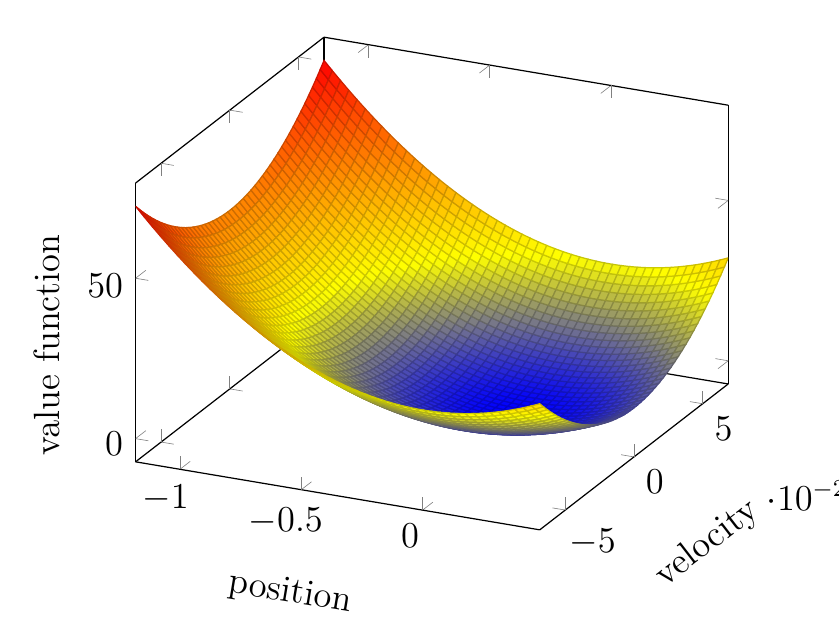
\includegraphics[scale=0.21]{basisval.jpeg}
$\mbox{ }$
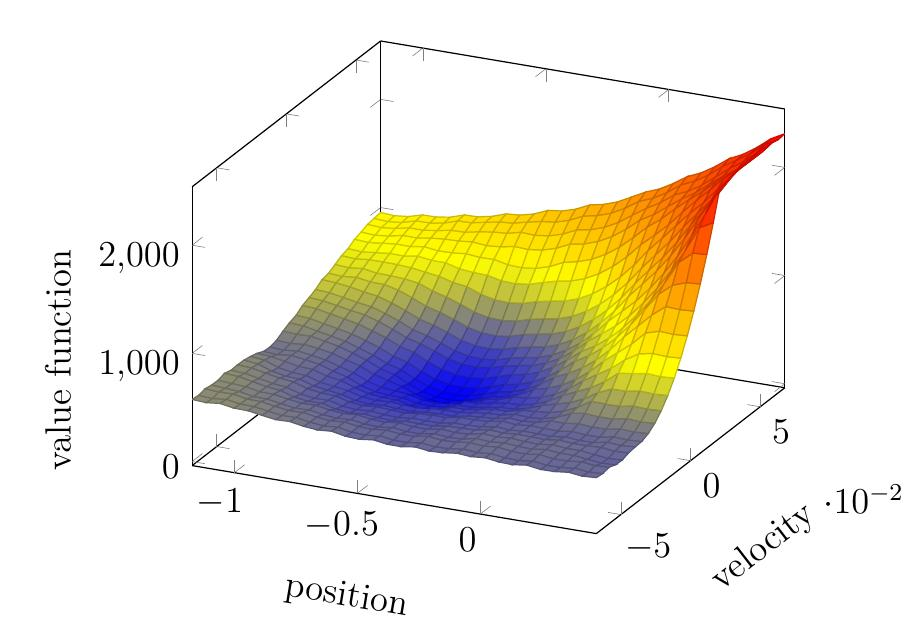
\includegraphics[scale=0.19]{appval.jpeg}
\end{block}
\begin{tikzpicture}[overlay]
\node[orange] at (2,8.5) {Mountain Car};
\node[orange] at (8,8.5) {Exact Value};

\node[orange] at (2,4.5) {Basis};
\node[orange] at (8,4.5) {Approximate Value};
\end{tikzpicture}
\end{frame}



\end{document}
